
%(BEGIN_QUESTION)
% Copyright 2014, Tony R. Kuphaldt, released under the Creative Commons Attribution License (v 1.0)
% This means you may do almost anything with this work of mine, so long as you give me proper credit

Calculate the current drawn by the resistor and inductor in this AC circuit, as well as the source current.  You may express each of these quantities as a scalar number (i.e. no need to use rectangular or polar notation):

$$\includegraphics[width=15.5cm]{i01092x01.eps}$$

$I_R$ = \hskip 100pt $I_L$ = \hskip 100pt $I_{source}$ = 

\vskip 10pt

\underbar{file i01092}
%(END_QUESTION)





%(BEGIN_ANSWER)

$I_R$ = 166.7 mA \hskip 100pt $I_L$ = 397.9 mA \hskip 100pt $I_{source}$ = 431.4 mA

%(END_ANSWER)





%(BEGIN_NOTES)

{\bf This question is intended for exams only and not worksheets!}.

%(END_NOTES)


